\definecolor{col000}{rgb}{1,0.060,0}
\definecolor{col001}{rgb}{1,0.036,0}
\definecolor{col002}{rgb}{1,0.910,0}
\definecolor{col003}{rgb}{1,0.994,0}
\definecolor{col010}{rgb}{1,0.000,0}
\definecolor{col011}{rgb}{1,0.003,0}
\definecolor{col012}{rgb}{1,0.910,0}
\definecolor{col013}{rgb}{1,0.994,0}
\definecolor{col020}{rgb}{1,0.000,0}
\definecolor{col021}{rgb}{1,0.003,0}
\definecolor{col022}{rgb}{1,0.910,0}
\definecolor{col023}{rgb}{1,0.994,0}
\definecolor{col030}{rgb}{1,0.000,0}
\definecolor{col031}{rgb}{1,0.003,0}
\definecolor{col032}{rgb}{1,0.910,0}
\definecolor{col033}{rgb}{1,0.994,0}
\definecolor{col040}{rgb}{1,0.000,0}
\definecolor{col041}{rgb}{1,0.000,0}
\definecolor{col042}{rgb}{1,0.000,0}
\definecolor{col043}{rgb}{1,0.000,0}

 
\begin{figure}[!htb]
  \centering
  %\begin{subfigure}[b]{0.15\textwidth}
    \begin{tikzpicture}[scale=1.0,auto,swap]

    % the two brain figures on top
    \node (upper_brain) at (0,1.5) { \includegraphics*[scale=\scaleBrainImg,trim=0 0 240 0]{images/mriCog14Sim2PCA/stage_2.eps}};
    \node (lower_brain) at (0,-1.5) { \includegraphics*[scale=\scaleBrainImg,trim=240 0 0 0]{images/mriCog14Sim2PCA/stage_2.eps}};
    \node[above=0cm of upper_brain] (stage) {Stage 2};
    % the balls
    \draw[fill=col000] (-1.6,-3.4) circle [radius=0.33cm] node {\scriptsize W};
    \draw[fill=col001] (-0.7,-3.4) circle [radius=0.33cm] node {\scriptsize A};
    \draw[fill=col002] (0.2,-3.4) circle [radius=0.33cm] node {\scriptsize V};
    \draw[fill=col003] (-1.6,-4.2) circle [radius=0.33cm] node {\scriptsize F};
    
    \end{tikzpicture}
  %\end{subfigure}
  % next subfigure
  \hspace{-1.5em}
  ~
  %\begin{subfigure}[b]{0.15\textwidth}
    \begin{tikzpicture}[scale=1.0,auto,swap]

    % the two brain figures on top
    \node (upper_brain) at (0,1.5) { \includegraphics*[scale=\scaleBrainImg,trim=0 0 240 0]{images/mriCog14Sim2PCA/stage_5.eps}};
    \node (lower_brain) at (0,-1.5) { \includegraphics*[scale=\scaleBrainImg,trim=240 0 0 0]{images/mriCog14Sim2PCA/stage_5.eps}};
    \node[above=0cm of upper_brain] (stage) {Stage 5};
    % the balls
    \draw[fill=col010] (-1.6,-3.4) circle [radius=0.33cm] node {\scriptsize W};
    \draw[fill=col011] (-0.7,-3.4) circle [radius=0.33cm] node {\scriptsize A};
    \draw[fill=col012] (0.2,-3.4) circle [radius=0.33cm] node {\scriptsize V};
    \draw[fill=col013] (-1.6,-4.2) circle [radius=0.33cm] node {\scriptsize F};
    
    \end{tikzpicture}
  %\end{subfigure}
  % next subfigure
  \hspace{-1.5em}
  ~
  %\begin{subfigure}[b]{0.15\textwidth}
    \begin{tikzpicture}[scale=1.0,auto,swap]

    % the two brain figures on top
    \node (upper_brain) at (0,1.5) { \includegraphics*[scale=\scaleBrainImg,trim=0 0 240 0]{images/mriCog14Sim2PCA/stage_8.eps}};
    \node (lower_brain) at (0,-1.5) { \includegraphics*[scale=\scaleBrainImg,trim=240 0 0 0]{images/mriCog14Sim2PCA/stage_8.eps}};
    \node[above=0cm of upper_brain] (stage) {Stage 8};
    % the balls
    \draw[fill=col020] (-1.6,-3.4) circle [radius=0.33cm] node {\scriptsize W};
    \draw[fill=col021] (-0.7,-3.4) circle [radius=0.33cm] node {\scriptsize A};
    \draw[fill=col022] (0.2,-3.4) circle [radius=0.33cm] node {\scriptsize V};
    \draw[fill=col023] (-1.6,-4.2) circle [radius=0.33cm] node {\scriptsize F};
    
    \end{tikzpicture}
  %\end{subfigure}
  % next subfigure
  \hspace{-1.5em}
  ~
  %\begin{subfigure}[b]{0.15\textwidth}
    \begin{tikzpicture}[scale=1.0,auto,swap]

    % the two brain figures on top
    \node (upper_brain) at (0,1.5) { \includegraphics*[scale=\scaleBrainImg,trim=0 0 240 0]{images/mriCog14Sim2PCA/stage_11.eps}};
    \node (lower_brain) at (0,-1.5) { \includegraphics*[scale=\scaleBrainImg,trim=240 0 0 0]{images/mriCog14Sim2PCA/stage_11.eps}};
    \node[above=0cm of upper_brain] (stage) {Stage 11};
    % the balls
    \draw[fill=col030] (-1.6,-3.4) circle [radius=0.33cm] node {\scriptsize W};
    \draw[fill=col031] (-0.7,-3.4) circle [radius=0.33cm] node {\scriptsize A};
    \draw[fill=col032] (0.2,-3.4) circle [radius=0.33cm] node {\scriptsize V};
    \draw[fill=col033] (-1.6,-4.2) circle [radius=0.33cm] node {\scriptsize F};
    
    \end{tikzpicture}
  %\end{subfigure}
  % next subfigure
  \hspace{-1.5em}
  ~
  %\begin{subfigure}[b]{0.15\textwidth}
    \begin{tikzpicture}[scale=1.0,auto,swap]

    % the two brain figures on top
    \node (upper_brain) at (0,1.5) { \includegraphics*[scale=\scaleBrainImg,trim=0 0 240 0]{images/mriCog14Sim2PCA/stage_14.eps}};
    \node (lower_brain) at (0,-1.5) { \includegraphics*[scale=\scaleBrainImg,trim=240 0 0 0]{images/mriCog14Sim2PCA/stage_14.eps}};
    \node[above=0cm of upper_brain] (stage) {Stage 14};
    % the balls
    \draw[fill=col040] (-1.6,-3.4) circle [radius=0.33cm] node {\scriptsize W};
    \draw[fill=col041] (-0.7,-3.4) circle [radius=0.33cm] node {\scriptsize A};
    \draw[fill=col042] (0.2,-3.4) circle [radius=0.33cm] node {\scriptsize V};
    \draw[fill=col043] (-1.6,-4.2) circle [radius=0.33cm] node {\scriptsize F};
    
    \end{tikzpicture}
  %\end{subfigure}
  % next subfigure
  \hspace{-1.5em}
  ~
  \hspace{1em}
  % the red-to-yellow gradient on the right
  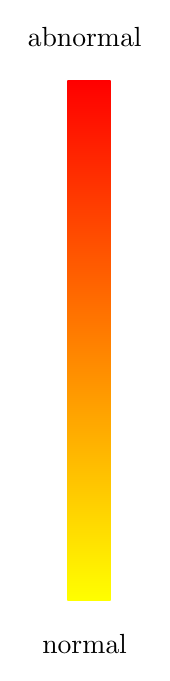
\begin{tikzpicture}[scale=1.1,auto,swap]
    \shade[top color=red,bottom color=yellow] (0,0) rectangle (0.5,6);
    \node[inner sep=0] (corr_text) at (0.2,6.5) {abnormal};
    \node[inner sep=0] (corr_text) at (0.2,-0.5) {normal};
  \end{tikzpicture}
  \caption[Atrophy progression snapshots for PCA subjects using imaging and cognitive biomarkers]{Atrophy progression snapshots for the PCA subjects at several informative stages in the disease: 2,5,8,11 and 14. Each brain region is coloured from yellow to red, according to how abnormal it is at that stage. The 4 circles underneath the brain picture represent cognitive biomarkers: W - RMT words, A - Arithmetic, V - VOSP OD, F - RMT faces. The positional variance matrix used is the one from sampling method 2 from figure \ref{fig:mriCog14_simult2L}. The model suggests that in PCA patients cognitive tests such as RMT words and Arithmetic become abnormal first, followed by middle occipital area, superior parietal lobule and occipital fusiform gyrus. }
  \label{fig:snap_mriCog14_sim2_pca}
\end{figure}